\begin{figure}
    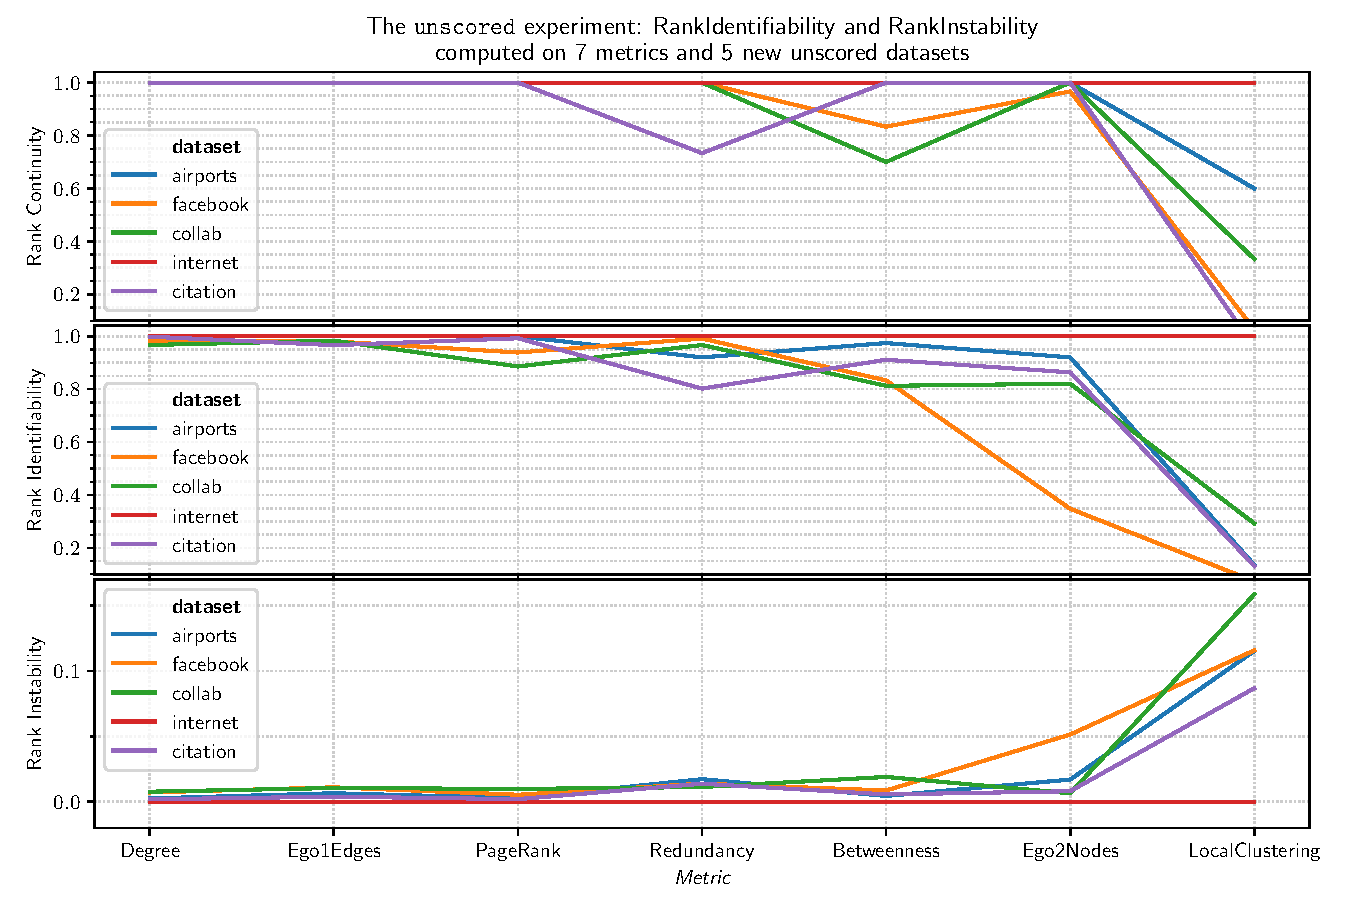
\includegraphics[width=\linewidth]{plot_unscored.pdf}
    \vspace*{-0.6cm}
    \caption{Evaluating RankContinuity, RankIdentifiability and RankInstability on 5 new unscored datasets, generating graphs by randomly deleting $4\%$ of edges.}
    \label{fig:plot_unscored}
    \footnotesize\justify\vspace{-0.4\baselineskip}
    High values of RankContinuity and RankIdentifiability mean high robustness, whereas high values of RankInstability mean low robustness.
    Metrics are sorted from left to right by their decreasing combined robustness.
\end{figure}
